This section provides background on operating system terminologies such as Processes, Threads, Memory Protection, Virtualization and Hypervisors.
\section{Processes and Threads}
\paragraph{Process:} A process can be viewed as a program in execution as an abstraction of a processor. Each process has its own address space.~\cite{Galvin}.

\paragraph{Threads:} A process has either a single or multiple threads sharing its address space. Each thread represents a separate flow of control~\cite{Galvin}.
\\[3mm]
A thread is also called a light-weight process. The implementation of threads and processes differs between operating systems. Multiple threads can exist within the same process and share resources such as code and data segments, whereas different processes do not share such resources. 
\begin{figure}[!ht]
    \centering
    \begin{subfigure}[b]{0.45\textwidth}
	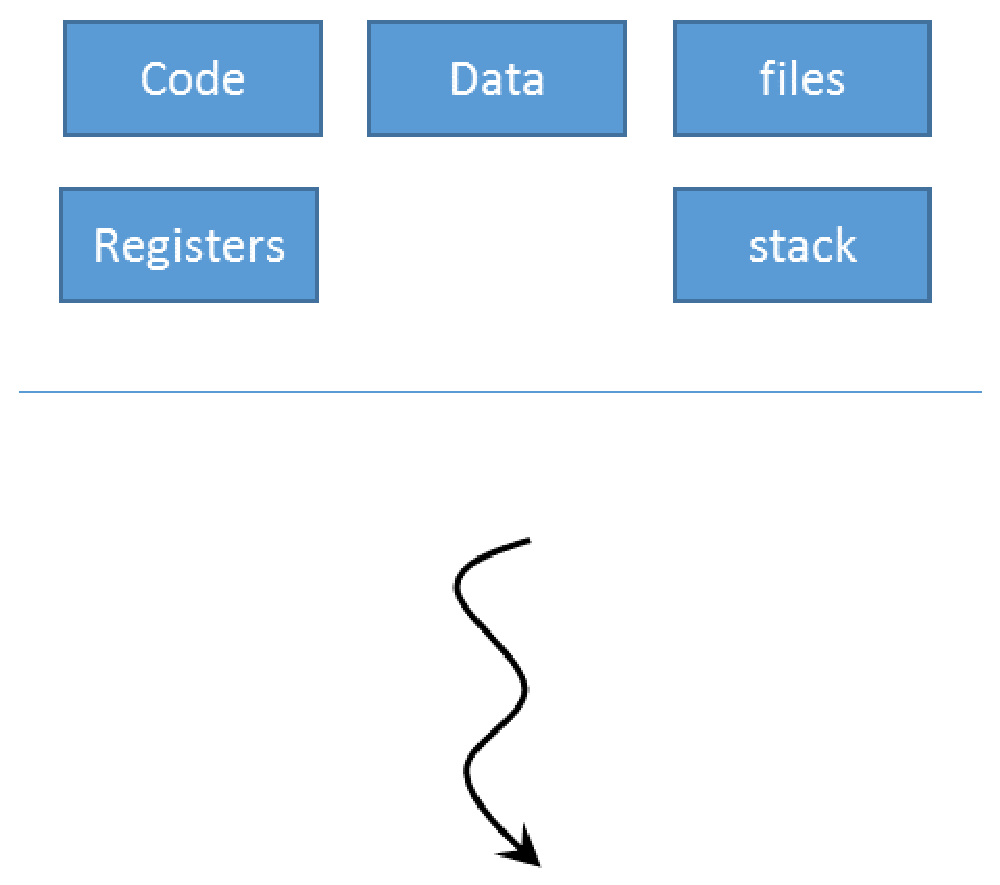
\includegraphics[scale=.25]{thread1}
	\caption{Single threaded process}
	\label{fig:thread1}
    \end{subfigure}
	\hfill
    \begin{subfigure}[b]{0.45\textwidth}
	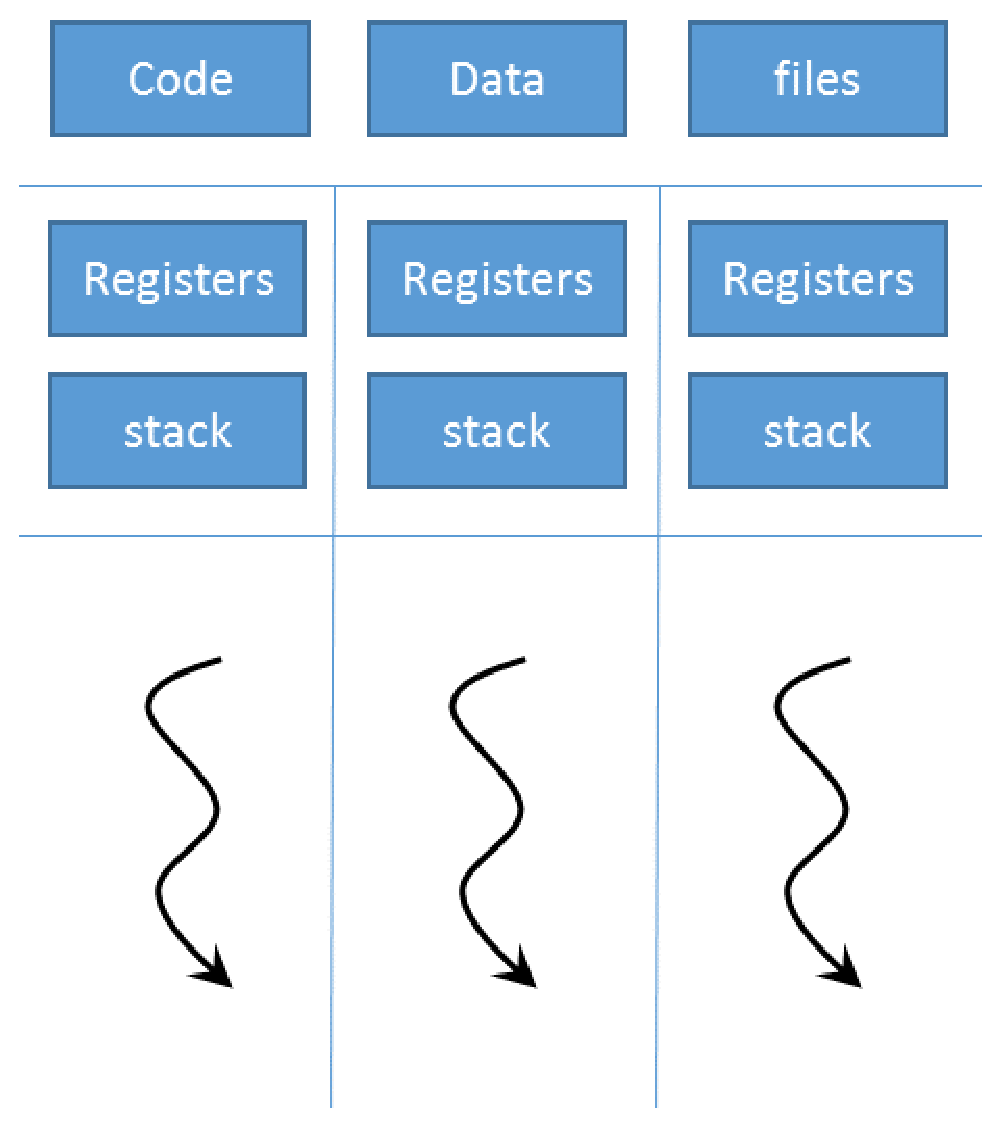
\includegraphics[scale=.25]{thread2}
	\caption{Multithreaded process}
	\label{fig:thread2}
    \end{subfigure}
    \caption{Thread}\label{fig:threads}
\end{figure}

\section{Context Switch}
Multiple threads typically employs time division multiplexing when sharing a single processor. In time division multiplexing, the processor switches between executing threads, interleaving their execution. Switching between threads is called a context switch. Continuous context switching creates the impression for the user that threads and processes are running concurrently. On multi-processor systems, threads can run simultaneously on multiple processors, each of which may perform time division multiplexing. 
\\[3mm]
Suring a context switch the state of a process is saved, so that its execution can be resumed from the same point at a later time. The state is determined by the processor and the operating system ~\cite{Galvin}. The cost of context switch can be divided into direct and indirect cost. The direct cost is the time required to save and restore processor registers, execute the scheduler code, flush TLB entries and flush pipeline. The indirect cost is the time spent due to processor pollution~\cite{Soares+:osdi10, Li:2007:QCC:1281700.1281702}.

\section{Spinlocks}
In uniprocessor and multiprocessor environment, a context switch takes a significant amount of time. In a multi-processor environment, it is more efficient for each process to keep its own CPU and spin while waiting for a resource~\cite{Bovet:2005:ULK:1077084}.
\\[3mm] 
A spinlock is a locking mechanism designed to work in a multi-processing environment. A spinlock causes a thread that is trying to acquire lock to spin if the lock is not available~\cite{Bovet:2005:ULK:1077084}.
\\[3mm]
\textbf{Adaptive Spinning} is a spinlock optimization technique. In the adaptive spinning technique, the duration of spinning is determined by algorithm based on the rate of successes and failures of recent spinning attempts to acquire the lock. Adaptive spinning helps threads to avoid spinning in unnecessary conditions.

\section{Device Driver}
\label{sec:device driver}
A device driver is a program that provides a software interface to a particular hardware device. It enables the operating system and other programs to access its hardware functions. Device drivers are hardware dependent and operating system specific. For a system call requested by a user program, a driver issues commands to the device. After execution, the device sends data back to the driver. The driver may invoke routines in the original calling program after receiving the data. The Linux kernel distinguishes between three device types: character devices, block devices and network interfaces. 
\begin{figure}[!ht]
\centering
\includegraphics[scale=.5 ]{kernel}
\caption{Split view of a kernel}
\label{fig:kernel}
\end{figure}
\paragraph{Character devices:} A character device can be accessed as a stream of bytes. A character driver usually implements at least the open, close, read, and write functions. The text console (/dev/console) and the serial ports (/dev/ttyS0) are examples of character devices.

\paragraph{Network Interfaces:} A network interface is a device that is able to exchange data with other hosts. Usually, a network interface is a hardware device, but it can be a software device like the loopback interface. 

\paragraph{Block Devices:} Unlike character devices, block devices are accessed as blocks of data. In most unix implementations, a block device can only handle I/O operations that transfer one or more whole blocks. Linux, instead, allows the application to read and write any number of bytes on a block device. As a result, block and char devices differ only in the way data is managed internally by the kernel. Examples of block devices are disks and CDs~\cite{Corbet:2005:LDD:1209083}.

\subsection*{Block Device Driver}
\subsubsection*{Request processing in a block device driver}
\label{subsec:request queue}
A block device driver maintains a request queue to store read, write requests. In order to initialize a request queue, a spinlock and a request function pointer is required. Request function is considered as a central part of the block device driver. Requests are added to the request queue when a request is made by higher level code in the Linux kernel, such as File systems. A block device driver calls its request function after receiving a new request. The request function removes all requests from the head of the request queue and sends them to the block device for execution. The Linux kernel acquires a spinlock before execution of the request function and releases it after completing execution. As a result, a request function runs in an atomic context~\cite{Corbet:2005:LDD:1209083}.
\\[3mm]
A request is a linked list of \textbf{bio structures}. A bio structure contains all the information required to execute a read and write operation on a block device. The block I/O code receives the bio structure from the higher level code in the Linux kernel. The block I/O code adds the received bio structure into existing request~\cite{Corbet:2005:LDD:1209083}.
\\[3mm]
Each bio structure in a request describes the low level block I/O request. If possible, the Linux kernel merges several independent requests to form one block I/O request. Usually the kernel combines multiple requests if they requires access to the adjacent sectors on the disk. However, it never combines a read and write request together.

\section{Memory Protection}
The memory protection mechanism of a computer system controls access to resources. The goal of memory protection is to prevent malicious misuse of the system by users or programs. Memory protection also ensures that a resource is used in accordance with the system policies. In addition, it also helps to ensure that errant programs cause minimal damage~\cite{Galvin, Graham:1971:PPP:1478873.1478928}. Subsection~\ref{subsec:user level} and subsection~\ref{subsec:kernel level} explain the policies implemented at kernel level and user level. 

\subsection{User Level}
\label{subsec:user level}
Typically in a monolithic kernel, the lowest \texttt{X Gb} of memory is reserved for user processes. The upper \texttt{Virtual Memory size - X Gb} is reserved for the kernel. The kernel puts its private data structures in the upper memory and always accesses them at the same virtual address. 
\begin{figure}[!ht]
\centering
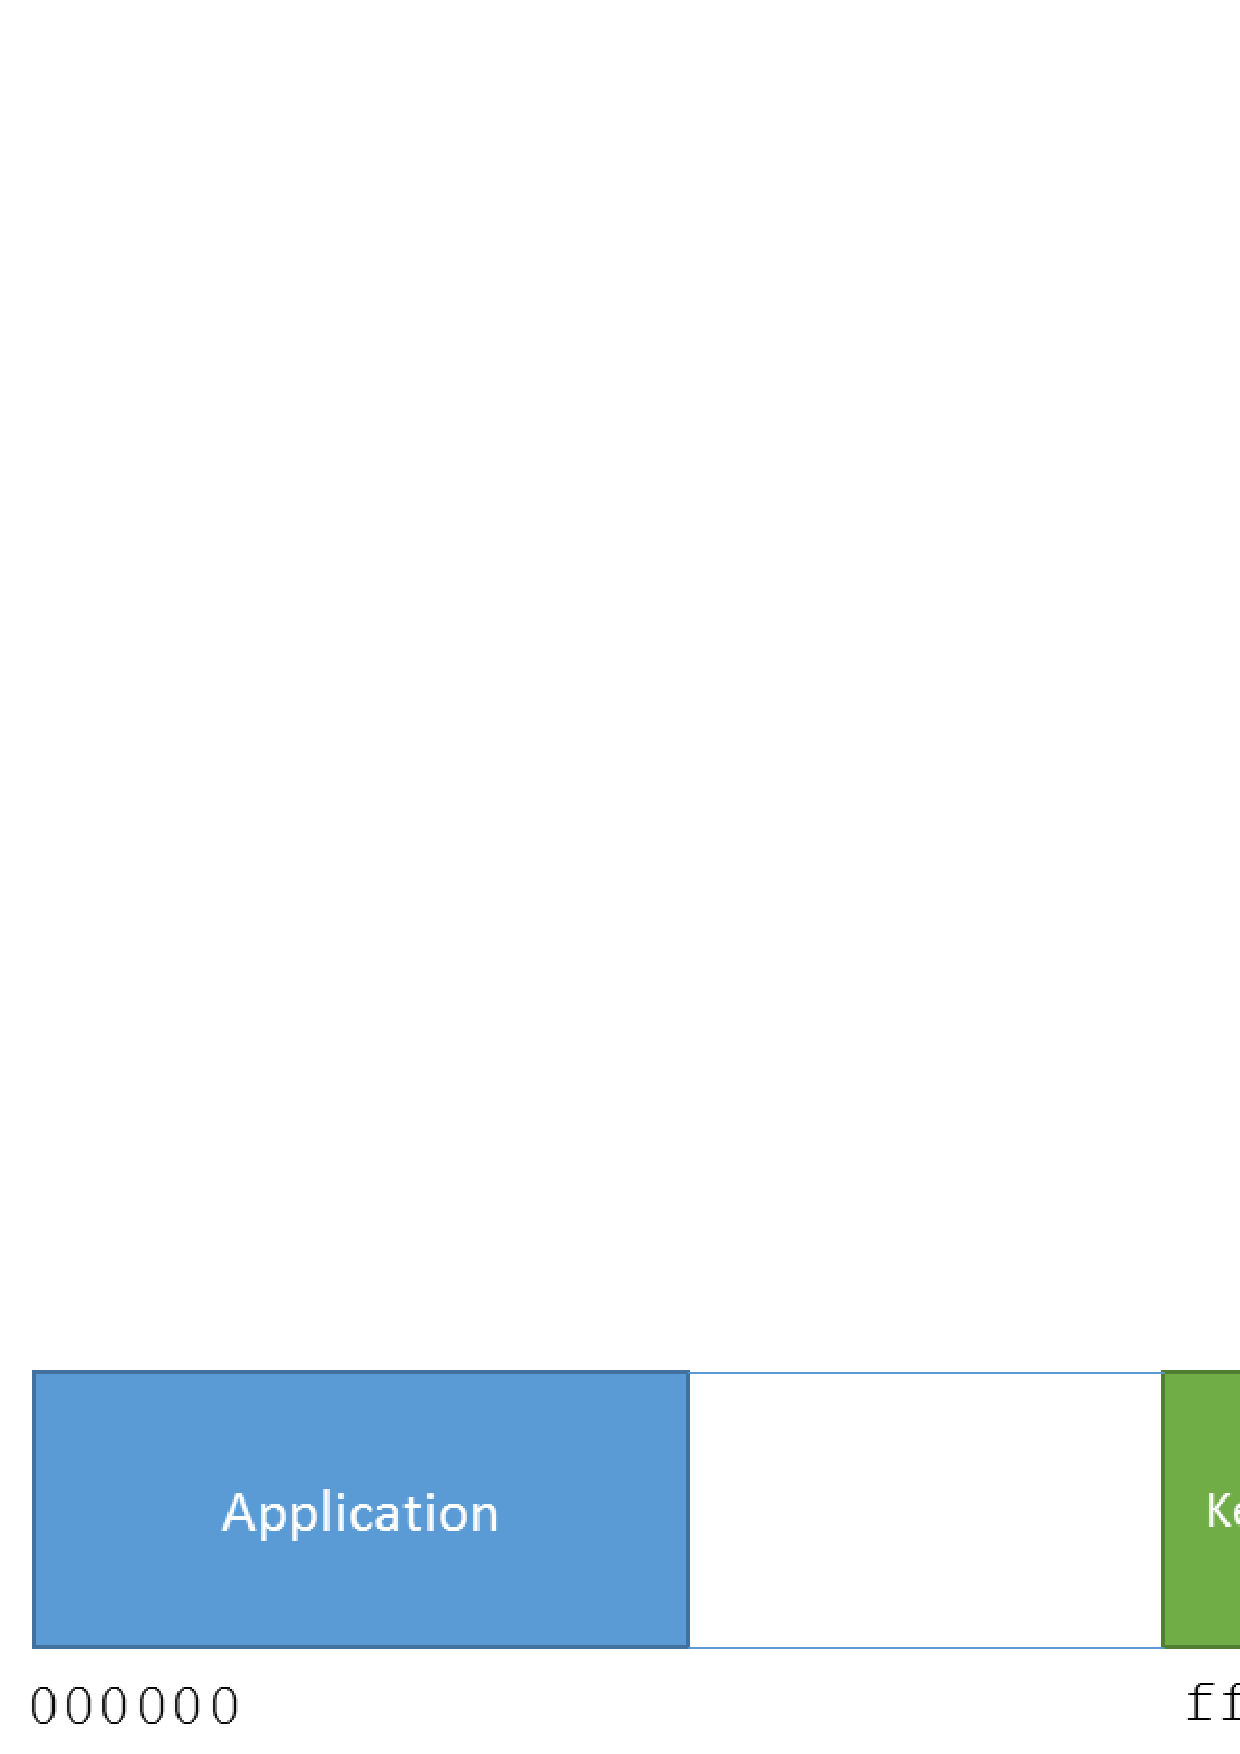
\includegraphics[scale=.25 ]{memory_map}
\caption{Physical memory}
\label{fig:memmap}
\end{figure}
\\[3mm]
At the user space, each application runs as a separate process. Each process is associated with an address space and believes that it owns the entire memory, starting with the virtual address 0. However, a translation table translates every memory reference by these processes from virtual to physical addresses. The translation table maintains \texttt{$<$base, bound$>$} entries. If a process tries to access virtual address that is outside the \texttt{base + bound} address, then an error is reported by the operating system, otherwise the physical address \texttt{base + virtual address} is returned. This allows multiple processes to be run in the memory with protection. Since address translation provides protection, a process can not access addresses outside its address space.
\\[3mm]
Consider the example shown in Figure~\ref{fig:User space}.
\begin{enumerate}
\item This system is running 3 different user processes
\item One of the processes encounters a bug and tries to access a memory address outside its address space
\item Access to the address is restricted by the memory protection mechanism
\begin{figure}[!ht]
    \centering
    \begin{subfigure}[b]{0.49\textwidth}
	\includegraphics[scale=.25]{user-space-1}
	\caption{A process encounters a bug}
    \end{subfigure}
	\hfill
    \begin{subfigure}[b]{0.49\textwidth}
	\includegraphics[scale=.25]{user-space-2}
	\caption{Other user processes are not affected}
    \end{subfigure}
    \caption{User level memory protection}\label{fig:User space}
\end{figure}
\end{enumerate}

\subsection{Kernel Level}
\label{subsec:kernel level}
This sections explains the memory management at kernel level. 
\\[3mm]
In a Linux kernel physical memory is divided into blocks called as page frames and virtual memory is divided into pages. Linux kernel uses a data structure called page table to store the virtual memory to physical memory mapping information. Kernel reserves upper virtual memory for its internal use. The page table entries of this region are marked as protected so that pages are not visible or modifiable in the user mode. This reserved region is divided into two parts. The first part contains references in a page table to every page in the system. It is used to do translations of addresses from physical to virtual when the kernel code is executed. The core of the kernel and all the pages allocated by page allocator lies in this region. The other region of the kernel memory is used by the memory allocator, the allocated memory is mapped by kernel modules. Since an operating system maps physical addresses directly, kernel components do not have memory protection similar to that of the user space. At kernel level any code running at \texttt{CPL 0} can access the kernel memory, hence a kernel component can access, and potentially, corrupt the kernel data structures. 
\\[3mm]
Consider an example shown in the Figure~\ref{fig:Kernel space}.
\begin{enumerate}
\item The system runs 3 different processes in the user space and has different kernel components running in the kernel space.
\item The network driver hits a bug, and corrupts the kernel data structure. The corruption might lead to a system crash.
\end{enumerate}
\begin{figure}[!ht]
    \centering
    \begin{subfigure}[b]{0.49\textwidth}
	\includegraphics[scale=.25]{kernel-space-1}
	\caption{A kernel component hits a bug}
    \end{subfigure}
	\hfill
    \begin{subfigure}[b]{0.49\textwidth}
	\includegraphics[scale=.25]{kernel-space-2}
	\caption{Results in a system crash}
    \end{subfigure}
    \caption{Kernel level memory protection}\label{fig:Kernel space}
\end{figure}

\section{Virtualization}
Virtualization is the act of creating a virtual version of a hardware platform, storage device, or computer network resource etc. In an operating system virtualization, the software allows a hardware to run multiple operating system images at the same time.
\\[3mm]
Virtualization has the capability to share the underlying hardware resources and still provide an isolated environment to each operating system. In virtualization, each operating system runs independently from the other on its own virtual processors. Because of this isolation the failures in an operating system are contained. Virtualization is implemented in many different ways. It can be implemented either with or without hardware support. Also operating systems might require some changes in order to run in a virtualized environment~\cite{Drepper:2008:CV:1348583.1348591}. It has been shown that virtualization can be utilized to provide better security and robustness for operating systems~\cite{Fraser04safehardware, LeVasseur04UnmodifiedDriverReuse, Riley:2008:GPK:1433006.1433008}.
\begin{figure}[!ht]
    \centering
    \begin{subfigure}[b]{0.49\textwidth}
	\includegraphics[scale=.25]{OS-arch}
	\caption{Operating System Architecture}
	\label{fig:OS}
    \end{subfigure}
	\hfill
    \begin{subfigure}[b]{0.49\textwidth}
	\includegraphics[scale=.25]{Virtualization}
	\caption{Virtualization}
	\label{fig:Virtualization}
	\end{subfigure}
    \caption{Comparision of a non-virtualized system and a virtualized system}\label{fig:Kernel space}
\end{figure}

\subsection{Hypervisor}
Hypervisor is a piece of computer software, firmware or hardware that creates and runs virtual machines. Operating system virtualization is achieved by inserting a hypervisor between the guest operating system and the underlying hardware. Most of the literature presents hypervisor synonymous to a virtual machine monitor (VMM). While, VMM is a software layer specifically responsible for virtualizing a given architecture, a hypervisor is an operating system with a VMM. The operating system may be a general purpose one, such as Linux, or it may be developed specifically for the purpose of running virtual machines~\cite{Agesen:2010:EXV:1899928.1899930}.
\\[3mm]
A computer on which a hypervisor is running one or more virtual machines is defined as a host machine. Each virtual machine is called a guest machine. The hypervisor presents the guest operating systems with a virtual operating platform and manages the execution of the guest operating systems. Multiple instances of a variety of operating systems share the virtualized hardware resources. Among widely known hypervisors are Xen~\cite{barham2003xen, Chisnall:2007:DGX:1407351}, KVM~\cite{Habib:2008:VK:1344209.1344217, kivity2007kvm}, VMware ESX~\cite{Agesen:2010:EXV:1899928.1899930} and VirtualBox~\cite{camargos2008virtualization}.
\\[3mm]
There are two types of hypervisors~\cite{Goldberg:1973:AVM:800122.803950}
\begin{itemize}
\item Type 1 hypervisors are also called native hypervisors or bare metal hypervisors. Type 1 hypervisors run directly on the host's hardware to control the hardware and to manage guest operating systems. Type 1 hypervisors represent the classic implementation of virtual-machine architectures such as SIMMON, and CP/CMS. Modern equivalents include Oracle VM Server for SPARC, Oracle VM Server, the Xen hypervisor~\cite{barham2003xen}, VMware ESX/ESXi~\cite{Agesen:2010:EXV:1899928.1899930} and Microsoft Hyper-V.
\begin{figure}[!ht]
\centering
\includegraphics[scale=.35]{type1}
\caption{Type 1 hypervisors}
\label{Type 1 hypervisor}
\end{figure}
\item Type 2 hypervisors are also called hosted hypervisors. Type 2 hypervisors run within a conventional operating-system environment. VMware Workstation and VirtualBox are some examples of Type 2 hypervisors~\cite{Sugerman:2001:VID:647055.715774, camargos2008virtualization}.
\begin{figure}[!ht]
\centering
\includegraphics[scale=.4]{type2}
\caption{Type 2 hypervisors}
\label{fig:Type 2 hypervisor}
\end{figure}
\end{itemize}

\subsection{Xen Hypervisor}
Xen~\cite{barham2003xen} is a widely known Type 1 hypervisor that allows the execution of virtual machines in guest domains~\cite{king2003operating}. 
\\[3mm]
Xen runs guest operating systems in environments known as domains. \texttt{Domain 0} is the first guest to run, and has elevated privileges. Xen loads a \texttt{domain 0} guest kernel during boot. Unprivileged domain is called \texttt{domain U}. The Xen hypervisor does not include device drivers. Device management is included in privileged \texttt{domain 0}. \texttt{Domain 0} uses the device drivers present in the guest operating system. However, the other domains access devices using a split device driver architecture, in which a frontend driver in a guest domain communicates with a backend driver in \texttt{domain 0}.
\\[3mm]
Xen provides an inter-domain memory sharing API accessed through the guest kernel extensions and an interrupt-based inter-domain signaling facility called event channels to implement the efficient inter-domain communication. Split drivers use memory sharing APIs to implement I/O device ring buffers to exchange data across domains.
\\[3mm]
Figure~\ref{xen-split2} shows how an application running in a \texttt{domain U} guest writes data on a physical device. First, write request is sent to the file system. After that the frontend driver puts the data into memory which is shared between \texttt{domain 0} and \texttt{domain U}. The other half of the split device driver called the backend, running in the \texttt{domain 0} guest, reads the data from the buffer and sends it to the real device driver. The data is then written to the actual physical device~\cite{Chisnall:2007:DGX:1407351}.
\begin{figure}[!h]
\centering
\includegraphics[scale=.50]{xen-split-fs}
\caption{Xen split device driver}
\label{xen-split2}
\end{figure}
\\[3mm]
\begin{figure}[!h]
\centering
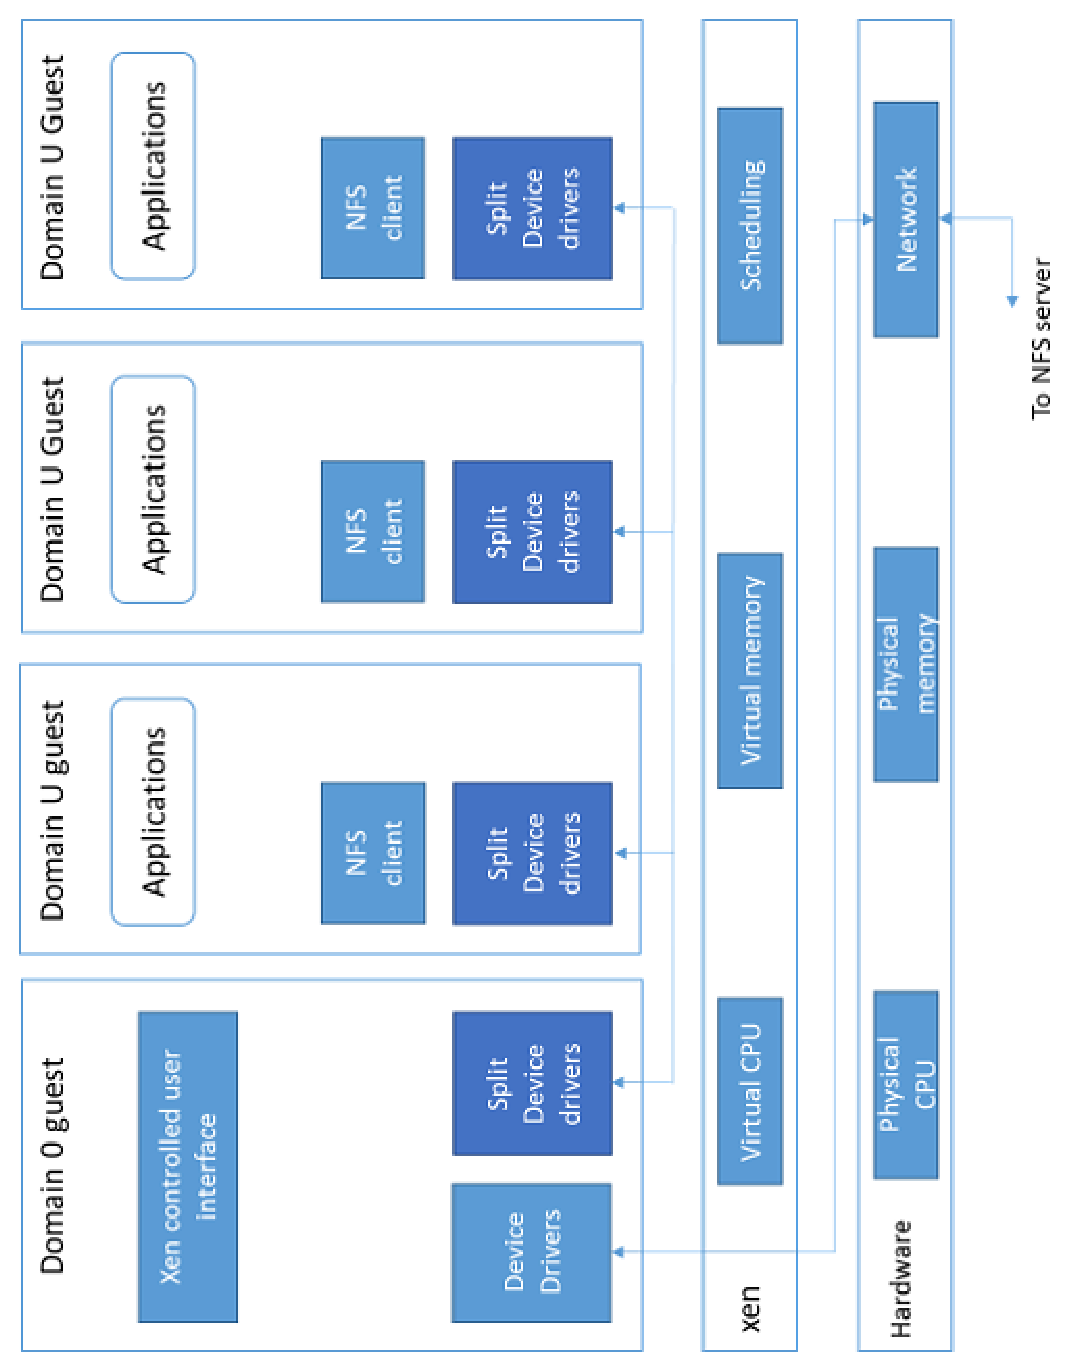
\includegraphics[scale=.50]{xen}
\caption{Xen}
\label{xen}
\end{figure}
\\[3mm]

\subsubsection*{Hypercalls and Events}
Hypercalls and event channels are the two mechanisms that exist for interactions between the Xen hypervisor and domains. A hypercall is a software trap from a domain to the Xen hypervisor, just as a syscall is a software trap from an application to the kernel~\cite{hypercall}. Domains use hypercalls to request privileged operations like updating pagetables. 
\\[3mm]
An event channel is to the Xen hypervisor as a signal is to an operating system. An event channel is used for sending asynchronous notifications between domains. Event notifications are implemented by updating a bitmap. After scheduling pending events from an event queue, the event callback handler is called to take appropriate action. The callback handler is responsible for resetting the bitmap of pending events and responding to the notifications in an appropriate manner. A domain may explicitly defer event handling by setting a Xen readable software flag: this is analogous to disabling interrupts on a real processor. Event notifications can be compared to traditional UNIX signals acting to flag a particular type of occurrence. For example, events are used to indicate that new data has been received over the network, or used to notify that a virtual disk request has completed. 

\subsubsection*{Data Transfer: I/O Rings}
\label{subsec:io rings}
Hypervisor introduces an additional layer between guest OS and I/O devices. Xen provides a data transfer mechanism that allows data to move vertically through the system with minimum overhead. 
\begin{figure}[!ht]
\centering
\includegraphics[scale=.5]{IObuffer}
\caption{Ring I/O buffer}
\label{fig:Ring buffer}
\end{figure}
\\[3mm]
Figure~\ref{fig:Ring buffer} shows the structure of an I/O descriptor ring. An I/O descriptor ring is a circular queue of descriptors allocated by a domain. These descriptors do not contain I/O data. However, I/O data buffers are allocated separately by the guest OS and is indirectly referenced by these I/O descriptors. Access to an I/O ring is based around two pairs of producer-consumer pointers.
\begin{enumerate}
\item Request producer pointer: A domain places requests on a ring by advancing a request producer pointer. 
\item Request consumer pointer: The Xen hypervisor removes requests pointed by a request producer pointer. These requests are removed by advancing a request consumer pointer.
\item Response producer pointer: The Xen hypervisor places responses on a ring by advancing a response producer pointer. 
\item Response consumer pointer: A domain removes responses pointed by a request producer pointer. These responses are removed by advancing a response consumer pointer.
\end{enumerate} 
The requests are not required to be processed in a specific order. I/O rings are generic to support different device paradigms. For example, a set of \texttt{requests} can provide buffers for read data of virtual disks; subsequent \texttt{responses} then signal the arrival of data into these buffers. 
\\[3mm]
The notification is not sent for production of each request and response. A domain can en-queue multiple requests and responses before notifying the other domain. This allows each domain to trade-off between latency and throughput.
\begin{figure}[!ht]
\centering
\includegraphics[scale=.5]{IObuffer2}
\caption{Ring I/O buffer}
\label{fig:Ring buffer}
\end{figure}

\subsection*{Shared Pages}
\label{subsec:sharedpages}
\subsubsection*{Grant Table} 
Grant tables are a mechanism provided by the Xen hypervisor for sharing and transferring frames between the domains. It is an interface for granting foreign access to machine frames and sharing memory between underprivileged domains provided by the Xen hypervisor. In Xen, each domain has a respective grant table data structure, which is shared with the Xen hypervisor. The grant table data structure is used by Xen to verify the access permission other domains have on the page allocated by a domain~\cite{granttable}.

\subsubsection*{Grant References}
Grant references are the entries in a grant table. A grant reference entry has every detail about the shared page. The Xen hypervisor virtualizes the physical memory, it is difficult to know the correct machine address of a frame for a domain. The biggest difficulty in sharing the memory between domains is knowing its correct machine address. A grant reference removes the dependency on the real machine address of the shared page. Hence, a grant entry makes it possible to share the memory between domains.\cite{Chisnall:2007:DGX:1407351, barham2003xen, granttable} 

\ifbool{toShowBibliography}{\bibliography{references}}{}
